\documentclass[12pt]{article}

\fontfamily{lmss}
\usepackage{fullpage}
\usepackage{amsmath}
\usepackage{amsthm}
\usepackage{url}
\usepackage{multicol}
\usepackage{enumerate}
\usepackage{graphicx}
\usepackage{color}

\usepackage{xcolor}

\usepackage{tikz}
\usetikzlibrary{graphs}
\usetikzlibrary{arrows.meta,shapes,shapes.geometric}
\usetikzlibrary{positioning, quotes}

\tikzset{
  % Two node styles for game trees: solid and hollow
  solid node/.style={circle,draw,inner sep=1.2,fill=black},
  hollow node/.style={circle,draw,inner sep=1.2},
  % styles for long branch labels
  left label/.style={above left,midway},
  right label/.style={above right,midway}
}

\usepackage{hyperref}
\hypersetup{
    colorlinks=true,
    linkcolor=blue,
    filecolor=magenta,      
    urlcolor=blue,
}

\usepackage{geometry}
\geometry{
  top=1in,            % <-- you want to adjust this
  bottom=1in,
  left=1in,
  right=1in,
  headheight=3ex,       % <-- and this
  headsep=4ex,          % <-- and this
}

\usepackage{lastpage}
\usepackage{fancyhdr}
\pagestyle{fancy}
\fancyhf{}
\renewcommand{\footrulewidth}{0.4pt}
\lhead{CS 486/686}
\rfoot{Page \thepage\ of \pageref{LastPage}}

\setlength{\parskip}{\baselineskip}%
\setlength{\parindent}{0pt}%

\usepackage{tcolorbox}
\tcbuselibrary{breakable}
\newenvironment{markscheme}
{
    \renewcommand{\parskip}{\baselineskip}
    \begin{tcolorbox}[
        colback=blue!10,
        colframe=blue!10,
        sharp corners,
        breakable
    ]
    \textbf{Marking Scheme:}
}
{
    \end{tcolorbox}
}

\newenvironment{sol}
{
    \renewcommand{\parskip}{\baselineskip}
    \begin{tcolorbox}[
        colback=magenta!10,
        colframe=magenta!10,
        sharp corners,
        breakable
    ]
    \textbf{Solutions:}
}
{
    \end{tcolorbox}
}


\lhead{CS 486/686}
\chead{Spring 2021}
\rhead{Assignment 1}
\lfoot{\copyright Ethan Yang}

\title{CS 486/686 Assignment 1 (140 marks)}
\author{Ethan Yang 20774734}

\hyphenation{PYTHONHASHSEED}

\usepackage{amsthm}
\usepackage{appendix}
\usepackage{pdfpages}

\begin{document}

\maketitle
\section*{Academic Integrity Statement}

I declare the following statements to be true:

\begin{itemize}
\item 
The work I submit here is entirely my own.

\item 	
I have not shared and will not share any of my code with anyone at any point. 

\item 
I have not posted and will not post my code on any public or private forum or website.

\item 	
I have not discussed and will not discuss the contents of this assessment with anyone at any point.

\item 
I have not posted and will not post the contents of this assessment and its solutions on any public or private forum or website. 

\item 
I will not search for assessment solutions online.

\item 
I am aware that misconduct related to assessments can result in significant penalties, possibly including failure in the course and suspension. This is covered in Policy 71: https://uwaterloo.ca/secretariat/policies-procedures-guidelines/policy-71.
\end{itemize}

Failure to accept the integrity policy will result in your assignment not being graded.

By typing or writing my full legal name below, I confirm that I have read and understood the academic integrity statement above.

{\bf\large Qianyu Yang}








\newpage
\section{The Wolves and Sheep Problem (42 marks)}

There are three wolves, three sheep, and a boat on the left side of the river. Let's assume that the wolves and sheep know how to row the boat. The boat can hold one or two animals. Every time the boat crosses the river, we count it as one boat trip. Our goal is to find a way to move all the animals from the left side to the right side of the river using the smallest number of boat trips subject to the constraints below. 
\begin{itemize}
\item
The boat can only cross the river if there is at least one animal in it. 
\item
The sheep must stay alive. 

At any moment in time, on either side of the river, if there is at least one sheep and the number of wolves is greater than the number of sheep, the wolves will eat the sheep.
\end{itemize}

You will apply uninformed and informed search algorithms to solve this problem. 

{\bf Please complete the following tasks.}

\begin{enumerate}[(a)]

%%%%%%%%%%%%%%%%%%%%%%%%%%%%%%%%%%%%%%%%%%%%%%%%%%%%%%%%%
%% SEARCH FORMULATION
%%%%%%%%%%%%%%%%%%%%%%%%%%%%%%%%%%%%%%%%%%%%%%%%%%%%%%%%%
\item
\label{mc_part_formulation}
Formulate this problem as a search problem. Make sure you define the states, the initial state, the goal state, the successor function, and the cost function.

In parts~\ref{mc_part_critique_formulation_1} and~\ref{mc_part_critique_formulation_2}, we will provide you with some other formulations. After that, you will have a chance to revise and improve your formulation in part~\ref{mc_part_formulation_improved}. Come up with your own formulation first before looking at the next two parts. Don't miss this valuable learning opportunity.

%%%%%%%%%%%%%%%%%%%%%%%%%%% Q1a
{\bf Answer:}

My formulation is as follow:

\begin{itemize}
\item
{\bf State:} Each state is given by $S_1 W_1 S_2 W_2 B$. $S_1$ and $W_1$ are the number of sheep/wolves on the start side and $S_2$ and $W_2$ are the number of sheep/wolves on the end side. $B = 0$ if the boat is on the start side and $B = 1$ if the boat is on the end side. The stat is valid if $S_i \geq W_i \geq 0$ or $W_i > S_i = 0$ for $i = 1, 2, \sum{S_i} = 3, \sum{W_i} = 3$

\item
{\bf Initial state:} $33000$ .

\item
{\bf Goal states:} $00331$.

\item
{\bf Successor function:} Assume A is a valid state and B is a successor of A. Then, start from A, we will move at least one, at most two animals from the side that the last digit of A represents, to the other side. Now, the boat is at the opposite side, therefore, the last digit of B will be different from A.

\item
{\bf Cost function:} The cost of each boat trip is one.
\end{itemize}



%%%%%%%%%%%%%%%%%%%%%%%%%%%%%%%%%%%%%%%%%%%%%%%%%%%%%%%%%
%% STATE DEFINITION
%%%%%%%%%%%%%%%%%%%%%%%%%%%%%%%%%%%%%%%%%%%%%%%%%%%%%%%%%
\item
\label{mc_part_critique_formulation_1}
Your friend Taylor came up with the following formulation. Taylor's formulation is correct, which means applying a (optimal) search algorithm on this formulation will allow us to find a (optimal) solution. Unfortunately, Taylor's formulation has a problem, which significantly affects the performance of a search algorithm on this problem. 

{\em Describe the problem with Taylor's formulation in no more than 3 sentences. Then, discuss how this problem affects the performance of a search algorithm in no more than a paragraph.}

Hint: If you have trouble identifying the problem, draw the search graph and look at the states in the search graph. How many states are there? Why are these states in the graph?

\begin{example}

{\bf Taylor's formulation:}
\begin{itemize}
\item
{\bf State:} Each state is given by $S_1 S_2 S_3 W_1 W_2 W_3 B$. $S_i$ and $W_j$ are 1 if the sheep/wolf is on the left bank and 0 otherwise. $B = d$ if the boat is on the left bank (departure side) and $B = a$ if the boat is on the right bank (arrival side). 

A state is valid if and only if it satisfies the following two constraints.

If there is at least one sheep on the left bank, then the number of wolves on the left bank must be less than or equal to the number of sheep on the left bank. 

If there is at least one sheep on the right bank, then the number of wolves on the right bank must be less than or equal to the number of sheep on the right bank. 

\item
{\bf Initial state:} $111111d$.

\item
{\bf Goal states:} Any state where every animal is on the right bank is a goal state. $000000x$ where $x$ can be $a$ or $d$.

\item
{\bf Successor function:} Assume that A and B are two states satisfying the state definition. B is a successor of A if and only if we can start from A, move the boat with one or two animals from one side of the river to the other side of the river, and arrive at state B.

\item
{\bf Cost function:} The cost of each boat trip is one.
\end{itemize}

\end{example}

%%%%%%%%%%%%%%%%%%%%%%%%%%% Q1b
{\bf Answer:}

The problem of Taylor's formulation is that it treats every sheep and wolf to be different among their own packs. This will lead to a lot of successors for a given state, and so there will be many states in the search graph.

The observed problem above will affect the space complexity since it creates more states. For a DFS algorithm, it will need to remember more states on each level, and for a BFS algorithm, on each level the branching factor will be larger hence the end level and above levels will have more states in total. This problem will also make BFS algorithm slower since BFS will expand all nodes on each level first and the branching factor is large.



%%%%%%%%%%%%%%%%%%%%%%%%%%%%%%%%%%%%%%%%%%%%%%%%%%%%%%%%%
%% CONSTRAINTS
%%%%%%%%%%%%%%%%%%%%%%%%%%%%%%%%%%%%%%%%%%%%%%%%%%%%%%%%%
\item
\label{mc_part_critique_formulation_2}
Your other friend Avery proposed a formulation that is similar to Taylor's. However, Taylor included the constraints in the state definition, whereas Avery put the constraints in the successor function. See the state and the successor function in the two formulations below.

Taylor and  Avery argued for a while but couldn't figure out which choice is better. Could you help them settle the argument? {\em Which of the two formulations is better? State your answer and justify your answer in no more than a paragraph.}

\begin{example}
{\bf Taylor's formulation:}

\begin{itemize}
\item
{\bf State:} Each state consists of $(S_1, S_2, S_3, W_1, W_2, W_3, B)$. $S_i$ and $W_j$ are 1 if the sheep/wolf is on the left bank and 0 otherwise. $B = d$ if the boat is on the left bank (departure side) and $B = a$ if the boat is on the right bank (arrival side). 

A state is invalid if it violates either constraint below.

\begin{itemize}
\item 
If there is at least one sheep on the left bank, then the number of wolves on the left bank must be less than or equal to the number of sheep on the left bank. 

\item
If there is at least one sheep on the right bank, then the number of wolves on the right bank must be less than or equal to the number of sheep on the right bank. 
\end{itemize}

\item
{\bf Successor function:} Assume that A and B are two states satisfying the state definition. B is a successor of A if and only if we can start from A, move the boat with one or two animals from one side of the river to the other side of the river, and arrive at state B. 

\end{itemize}

\end{example}

\begin{example}
{\bf Avery's formulation:}

\begin{itemize}
\item
{\bf State:} Each state consists of $(S_1, S_2, S_3, W_1, W_2, W_3, B)$. $S_i$ and $W_j$ are 1 if the sheep/wolf is on the left bank and 0 otherwise. $B = d$ if the boat is on the left bank (departure side) and $B = a$ if the boat is on the right bank (arrival side). 

\item
{\bf Successor function:} Consider a state A that satisfies the state definition. 
A does not have any successor if it violates either constraint below.

\begin{itemize}
\item 
If there is at least one sheep on the left bank, then the number of wolves on the left bank must be less than or equal to the number of sheep on the left bank. 

\item
If there is at least one sheep on the right bank, then the number of wolves on the right bank must be less than or equal to the number of sheep on the right bank. 
\end{itemize}

If state A satisfies both constraints above, then we will determine A's successor states as follows. Assume that B is a state satisfying the state definition. B is a successor of A if and only if we can start from A, move the boat with one or two animals from one side of the river to the other side of the river, and arrive at state B.
\end{itemize}

\end{example}


%%%%%%%%%%%%%%%%%%%%%%%%%%% Q1c
{\bf Answer:}

Taylor's formulation is better. The constraints should be included as part of the state definition. In Avery's formulation, if the constraints are in the successor function, there will be more states that will never exist in reality when we draw the search graph. Since those states satisfy the state definition, they will be a "valid" state and could be derived from its parent states. However, the search will terminate at them because of the reason that they cannot generate a successor instead of the reason that these states do not exist in the real world. Considering the complexity, those inexistent states will also lead to worse complexity. Therefore, Taylor's formulation is considered to be better.



\item
\label{mc_part_formulation_improved}

Based on the previous parts, come up with the best formulation for this problem. Make sure you define the states, the initial state, the goal state, and the successor function. Assume the cost function is the same as the one in Taylor's formulation. 

We will mark your formulation on its correctness and its quality.

%%%%%%%%%%%%%%%%%%%%%%%%%%% Q1d
{\bf Answer:}

My formulation is as follow:

\begin{itemize}
\item
{\bf State:} Each state is given by $(S_1 W_1 S_2 W_2 B)$. $S_1$ and $W_1$ are the number of sheep/wolves on the start side and $S_2$ and $W_2$ are the number of sheep/wolves on the end side. $B$ indicates the side of boat. $B = 0$ if the boat is on the start side and $B = 1$ if the boat is on the end side. The states must satisfy the following constraints: 
\begin{itemize}
\item $S_i \geq W_i \geq 0$ or $W_i > S_i = 0$ for $i = 1, 2$ (On both side, the number of sheep must be greater or equal to the number of wolves if there is at least one sheep), 
\item $\sum{S_i} = 3, \sum{W_i} = 3$ (There are 3 sheep and 3 wolves in total),
\item the boat side must have at least one animal (to use the boat) and cannot only have sheep (one or two sheep will die after using the boat to the other side).
\end{itemize}

\item
{\bf Initial state:} $33000$ .

\item
{\bf Goal states:} $00331$.

\item
{\bf Successor function:} Assume A is a valid state and B is a successor of A. Then, start from A, we will move at least one, at most two animals from the bank that the last digit of A represents, to the other side. Now, the boat is at the opposite bank, therefore, the last digit of B will be different from A.

\item
{\bf Cost function:} The cost of each boat trip is one.
\end{itemize}



%%%%%%%%%%%%%%%%%%%%%%%%%%%%%%%%%%%%%%%%%%%%%%%%%%%%%%%%%
%% SEARCH GRAPH
%%%%%%%%%%%%%%%%%%%%%%%%%%%%%%%%%%%%%%%%%%%%%%%%%%%%%%%%%
\item
\label{mc_part_graph}
Draw the search graph. The search graph should contain the states and the arcs in your problem formulation in part~\ref{mc_part_formulation_improved}. Highlight the start state and the goal states in your graph.

If you search graph has more than 35 nodes in it, go back to part~\ref{mc_part_formulation_improved} and rethink your formulation.

%%%%%%%%%%%%%%%%%%%%%%%%%%% Q1e
{\bf Answer:}
\begin{figure}[ht]
\centering
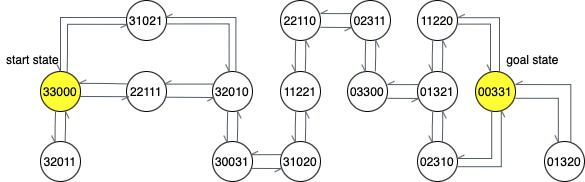
\includegraphics[width=0.8\textwidth]{a1q1e.png}
\caption{The search graph of my formulation in part(c)}
\label{a1q1d}
\end{figure}




%%%%%%%%%%%%%%%%%%%%%%%%%%%%%%%%%%%%%%%%%%%%%%%%%%%%%%
%%% CHOOSE UNINFORMED SEARCH ALGORITHM
%%%%%%%%%%%%%%%%%%%%%%%%%%%%%%%%%%%%%%%%%%%%%%%%%%%%%%
\item
If your goal is to find a solution quickly (while minimizing the number of nodes expanded), which {\bf uninformed search algorithm} would you use to solve this problem?

You can choose among breadth first search, depth first search, iterative-deepening search, and lowest-cost-first search. You can also use any pruning strategy discussed in lectures. Since you already drew the search graph, you can assume that it is given.

State the algorithm of your choice and justify your answer in at most 5 sentences.

%%%%%%%%%%%%%%%%%%%%%%%%%%% Q1f
{\bf Answer:}

I will choose a DFS algorithm with cycle pruning to find the solution for my formulation. From the search graph, it can be seen that the possible solution will be on a deep level. Compared to expanding on each level, I will prefer to go deeper. Since the cost function gives the same value for each arc, LCFS is the same as BFS, and I will choose DFS instead of other three algorithms. Also, since for all the states, the relations between the parent and successors are reversible, I will use cycle pruning to avoid trapped in cycle.




%%%%%%%%%%%%%%%%%%%%%%%%%%%%%%%%%%%%%%%%%%%%%%%%%%%%%%
%%% HEURISTIC FUNCTION
%%%%%%%%%%%%%%%%%%%%%%%%%%%%%%%%%%%%%%%%%%%%%%%%%%%%%%
\item
\label{mc_part_heuristic}

Propose an admissible heuristic function $h$. Describe the heuristic function in detail. Then, explain why the heuristic function is admissible. Some marks will be assigned to the quality of the heuristic function.

Hint: A heuristic function must specify a value for every state in the search graph.

Hint: If you relax the problem by removing a constraint, then the optimal solution to the relaxed problem is guaranteed to be an admissible heuristic function. One way to justify why your heuristic function is admissible is to explain how you relaxed the problem and solved the relaxed problem optimally. 

%%%%%%%%%%%%%%%%%%%%%%%%%%% Q1g
{\bf Answer:}

I will first give my heuristic function $h$ as follow:
\begin{equation}
 h(S_1W_1S_2W_2B) = 
 				\begin{cases}
				(S_1 + W_1) \cdot 2 - 1 & \text{if $B = 0$}\\
				(S_1 + W_1 + 1) \cdot 2 & \text{if $B = 1$}
				\end{cases}
\end{equation}

I get the heuristic function by relaxing the problem and obtain its optimal solution. Here is my detail explanation:

I remove the constraint that "On both side, the number of sheep must be greater or equal to the number of wolves if there is at least one sheep". Then, our problem becomes that all the animals should be moved from the start side to the end side. Now, if the boat is at the start side, then we will just move two animals to the end side and let one animal come back with the boat until there are only two animals left on the start side. Finally, we let that two animals go to the end side with 1 more cost. This will cost $(S_1 + W_1 - 1) \cdot 2 + 1 = (S_1 + W_1) \cdot 2 - 1$ in total, given that every boat trip costs 1. If the boat is at the end side, then we will first need one animal to take the boat back to the start side and then move all the animal to the end side. This will cost $1 + (S_1 + W_1 + 1 - 1) \cdot 2 + 1 = (S_1 + W_1 + 1) \cdot 2$. Therefore, the above process is the optimal solution for my relaxed problem and I obtain the corresponding heuristic function by calculating the cost of the optimal solution.

And since I obtain the heuristic function by getting the optimal solution to the relaxed problem, this heuristic function is admissible for my original formulation.




\item
Your friend is considering using {\bf the A* search algorithm} instead of using an uninformed search algorithm to solve the sheep and wolves problem. Would the A* search algorithm be a better choice than an uninformed search algorithm? Why or why not? State your answer and justify it in at most 5 sentences.

Tip: Do not trace the algorithm on the problem. We are not looking foxr the exact number of states expanded for either algorithm. Instead, formulate your answer by looking at the search graph and reasoning about the behaviour of the search algorithms.

%%%%%%%%%%%%%%%%%%%%%%%%%% Q1h
{\bf Answer:}

I think $A^{*}$ search algorithm will not be a better choice than an uninformed search algorithm with cycle pruning. From the search graph we can see that whenever there is state with three successors, one of the successors is its parent and the other two will be actually equivalent since they have a common successor. Therefore, every time $A^{*}$ make decisions of the sequences, the options are equivalent as long as the algorithm does not go into a cycle. If uninformed search does not have cycle pruning, then $A^{*}$ is better since it can avoid getting into the cycle.

\begin{markscheme}
(3 marks) A good justification for your answer.
\end{markscheme}


\end{enumerate}



\newpage
\section{The Rush Hour Sliding Puzzle (98 marks)}

In this programming question, you will solve the Rush Hour puzzle using the A* search and the depth-first search algorithms.

Take a look at an example of a Rush Hour puzzle below. The puzzle is on a 6 by 6 grid. We will number the rows as 0 to 5 from the top, and the columns as 0 to 5 from the left. In row 2, a horizontal car of length 2, called the goal car, is trying to escape through the exit on the right. There are horizontal and vertical cars of various lengths in the grid. A horizontal car can only move horizontally, whereas a vertical car can only move vertically. Each car may move more than one square in one step, but it cannot move over or through other cars. The goal is to move the cars around until the goal car reaches the exit, i.e. until the goal car is in the columns 4 and 5 in row 2. 

\begin{figure}[ht]
\centering
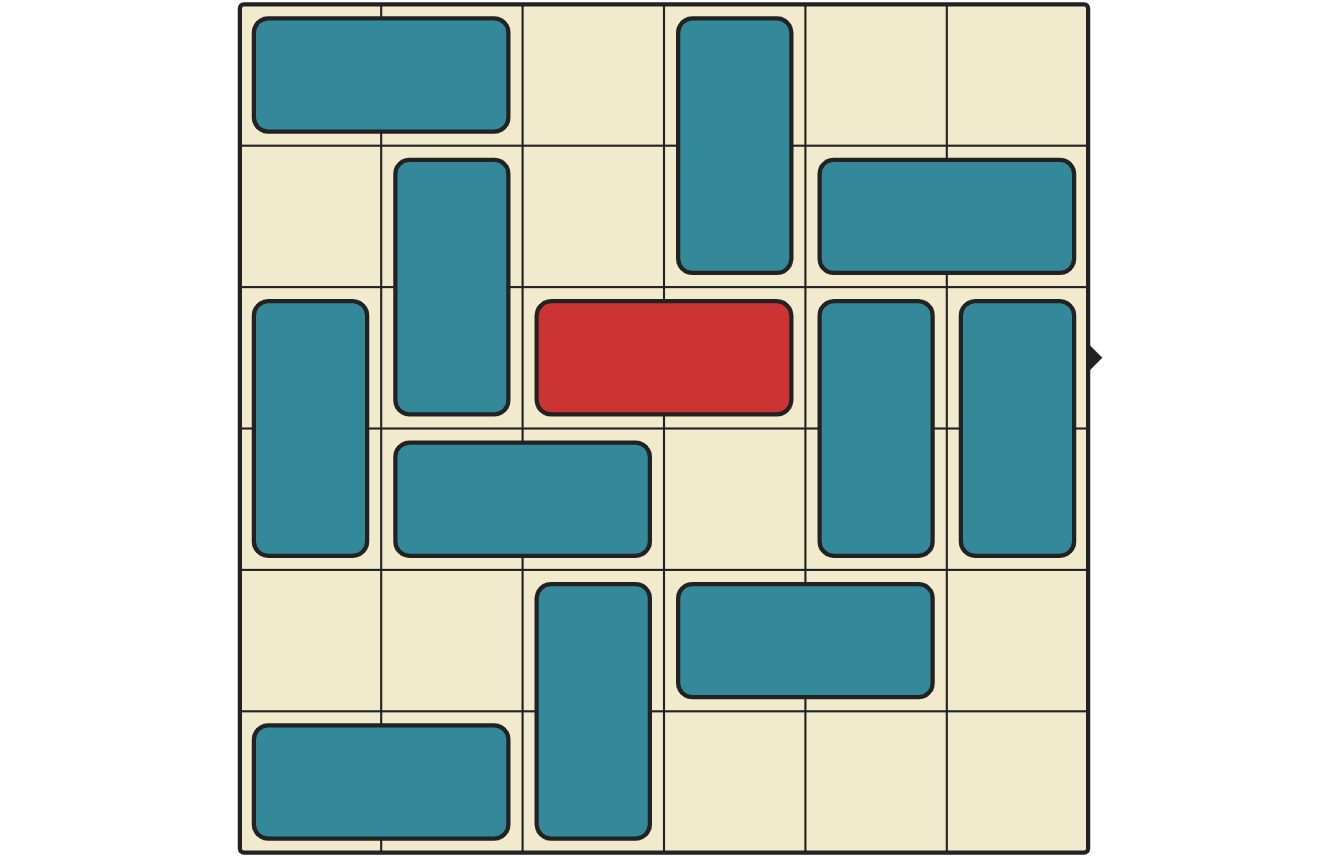
\includegraphics[width=0.7\textwidth]{images_posted/rush_hour_example.png}
\caption{An example of a Rush Hour puzzle from https://www.michaelfogleman.com/rush/}
\label{rush_hour_example}
\end{figure}

You can make the following assumptions for this question.
\begin{itemize}
  \item The puzzle must be on a 6 x 6 grid.
  \item The goal car is in row 2 and it has a length of 2.
  \item Besides the goal car, there is no other horizontal car in row 2.
\end{itemize}

{\bf Information on the Provided Code}

We have provided three files \verb+board.py+,  \verb+solve.py+, and \verb+jams_posted.txt+ on Learn. \verb+board.py+ contains code for handling input/output, representing states, etc. Your main task is to fill in the empty functions in \verb+solve.py+.

Submit the \verb+solve.py+ to Marmoset only. We will use our version of \verb+board.py+ to test your code. Do not modify any provided function signatures in \verb+solve.py+. Doing so will cause you to fail our tests. Feel free to add any new code to \verb+solve.py+. 

{\bf Input Format}

The file \verb+jams_posted.txt+ contains $40$ puzzles. You can use these puzzles to test your program. We will test your program using a different set of puzzles.

Below is an example of an input describing a puzzle.

\begin{verbatim}
example
6
1 2 h 2
2 0 v 2
4 0 h 2
3 1 v 3
4 1 v 2
4 3 h 2
.  
\end{verbatim}

\begin{itemize}
\item The first line assigns a name to the puzzle. In this case, the name is ``example.''
\item The next line specifies the size of the grid. We only use 6 by 6 grid. So this number is always 6.
\item The next line ``\verb+1 2 h 2+'' gives a description of the goal car.  The first two numbers $(1,2)$ gives the $(x,y)$ coordinates of the upper left corner of the car. The next letter ``h'' indicates that the car is horizontal (``v'' would indicate that the car is vertical). The last number ``2'' indicates that the car has size 2.
\item Each subsequent line, except the last line, describe a car in the puzzle, using the same format.
\item The last line consists of a single period, indicating the end of the puzzle. 
\end{itemize}

You can include multiple puzzles consecutively in the same file using the above format. 

{\bf The Heuristic Functions for A* Search:}

We have provided the implementation of the zero Heuristic function, which assigns a heuristic value of 0 to every state.

You must implement two other heuristic functions for A* search.
\begin{itemize}

  \item Blocking Heuristic: The heuristic value for any goal state is zero. For any non-goal state, the heuristic value is one plus the number of cars blocking the path to the exit. For example, for the state in Figure~\ref{rush_hour_example}, the blocking heuristic value is $3$.
  
  \item Advanced Heuristic: Implement a third advanced heuristic of your choosing and invention. Your advanced heuristic should be consistent and should dominate the blocking heuristic.
  
\end{itemize}

{\bf Testing Your Program}

Debugging and testing are essential skills for computer scientists. For this question, debugging your program may be especially challenging because of ties. Among ``correct'' implementations, the number of nodes expanded may vary widely due to how we handle the nodes with the same heuristic value on the frontier. 

Please test your code using {\bf Python 3.8.5}. 

{\bf We rely on Python's hashing to generate a state's ID for breaking ties} (see the Breaking Ties section below). However, Python' hashing function is not deterministic across different sessions. For example, you may get different hashing values of the same object for running your program multiple times. {\bf Please set the environment variable PYTHONHASHSEED to 486 BEFORE running the Python script.} Note that setting the variable in the code/program will not work.

Implement {\bf multi-path pruning for both DFS and A*}. When there are multiple paths to a state, multi-path pruning explores the first path to the state and discards any subsequent path to the same state. Use an explored set to keep track of the states that have been expanded by the algorithm. When you {\bf remove} a state from the frontier, check whether the state is in the explored set or not. If the state is in the explored set, then do nothing. Otherwise, add the state to the explored set and continue with the algorithm. Note that we perform pruning after we {\bf remove} a state from the frontier, not before we {\bf add} a state to the frontier.

DFS's behaviour depends on the order of adding a state's successors to the frontier. We will break ties by using the states' ID values. At each step, DFS will add the successors to the frontier in {\bf decreasing} order of their IDs. In other words, DFS will expand the state with the smallest ID value among the successors.

A* search will also break ties using the states' ID values. Among several states with the same $f$ value, A* will expand the state with the smallest ID value. If two states have the same ID value, A* will break ties using the states' parents --- expanding the state whose parent has the smaller ID value.

{\bf Please complete the following tasks:}

Submit your solutions to part (a) on Marmoset and submit your solutions to parts (b) and (c) on Learn.

\begin{enumerate}[(a)]

\item Complete the empty functions in \verb+solve.py+ and submit \verb+solve.py+ on \href{https://marmoset.student.cs.uwaterloo.ca/}{Marmoset}. Marmoset will evaluate your program for its correctness and efficiency.

For correctness, we have written unit tests for these functions: \verb+get_path+, \verb+is_goal+, \verb+blocking_heuristic+, \verb+get_successors+, \verb+dfs+, \verb+a_star+.

For each function, Marmoset provides one public test, which tests the function in a trivial scenario. There are also several secret tests. Before the deadline, you can only view the results of the public tests. After the deadline, Marmoset will run all the tests and calculate your marks.

Each test runs the function up to a predefined time limit. If the test passes if and only if the function terminates within the time limit and returns the expected result. Each test is all or nothing --- there are no partial marks available.

\begin{markscheme}
(88 marks) 

Unit tests on \verb+get_path+, \verb+is_goal+, \verb+blocking_heuristic+, \verb+get_successors+, \verb+dfs+, and \verb+a_star+. 

\begin{itemize}
\item \verb+get_path+: (1 public test + 2 secret tests) * 1 mark = 3 marks.
\item \verb+is_goal+:  (1 public test + 4 secret tests) * 1 mark = 5 marks.
\item \verb+blocking_heuristic+: (1 public test + 9 secret tests) * 2 marks = 20 marks.
\item \verb+get_successors+: (1 public test + 9 secret tests) * 2 marks = 20 marks.
\item \verb+dfs+:    (1 public test + 9 secret tests) * 2 marks = 20 marks.
\item \verb+a_star+: (1 public test + 9 secret tests) * 2 marks = 20 marks.
\end{itemize}

\end{markscheme}
  
\item Prove that the blocking heuristic is consistent using the definition of a consistent heuristic. 

%%%%%%%%%%%%%%%%%%%%%%%%%%% Q2b
{\bf Answer:}

\begin{proof}
Let $A$ be a valid state except the goal state, and $B$ be a successor of  $A$. Based on the blocking heuristic function, we can calculate $h(A)$ and $h(B)$. Then, the value of $h(A)$ and $h(B)$ represent the numbers of cars directly blocking the goal car. Additionally, we know that $B$ is the state that we take one more move on $A$. One additional move can at most remove one car that is blocking the goal car directly, which gives $h(A) - h(B) \leq 1$. Since we also know $cost(A,B) = 1$. We have
$$
h(A) - h(b) \leq cost(A, B)
$$
Therefore, by the definition of consistent heuristic, blocking heuristic is consistent.
\end{proof}



 
\item
Design and implement an advanced heuristic of your own invention. Your advanced heuristic should be consistent and dominate the blocking heuristic. 

Prove that your advanced heuristic is consistent and dominates the blocking heuristic.

Implement your advanced heuristic. Show that A* search with the advanced heuristic expands fewer nodes than A* search with the blocking heuristic on all the 40 provided puzzles.

%%%%%%%%%%%%%%%%%%%%%%%%%%% Q2c
{\bf Answer:}

Here is my advanced heuristic function: The heuristic value for any goal state is zero. For any non-goal state, the heuristic value is the heuristic value of blocking heuristic (i.e. one plus the number of cars directly blocking the goal car) plus one if among those cars directly blocking the goal car, there exists one car that is blocked by cars on both sides (i.e. this car cannot not move at this state).

\begin{proof}
For the state that "among those cars directly blocking the goal car, there exists one car among the cars directly blocking the goal car that is blocked by cars on both sides", the optimal solution is at least "free" the blocked car with one cost, remove all the cars directly blocking, and then move the goal car in addition one move. Thus, my heuristic value will always be less of equal to the cheapest cost to the goal state. It never overestimates. Therefore, my heuristic is admissible.

Now, Let $A$ be a valid state except the goal state, and $B$ be a successor of  $A$. Based on my advanced heuristic function, we can calculate $h(A)$ and $h(B)$. Then, the value of $h(A)$ and $h(B)$ represent one plus the numbers of cars directly blocking the goal car and plus one if any blocking car is blocked as well . One additional move can at most either remove one car that blocks the directly blocking car or remove one car that is blocking the goal car directly, which gives $h(A) - h(B) \leq 1$. Since we also know $cost(A,B) = 1$. We have
$$
h(A) - h(b) \leq cost(A, B)
$$
Therefore, my advanced heuristic is consistent by definition.

My advanced heuristic($h_1$) dominates blocking heuristic($h_2$) since for the states described above, $h_1 = h_2 + 1$. And for all other states, $h_1 = h_2$. Therefore, this satisfies:
$$
(\forall n (h_1(n) \geq h_2(n))) \wedge
(\exists n (h_1(n) > h_2(n)))
$$

Therefore, My advanced heuristic should dominate blocking heuristic.
\end{proof}

I have attached the program output of all 40 pairs of comparisons between advanced heuristic and blocking heuristic in the Appendices section. For all 40 boards, advanced heuristic expands less nodes than blocking heuristic, which support my proof above.



\end{enumerate}


\newpage
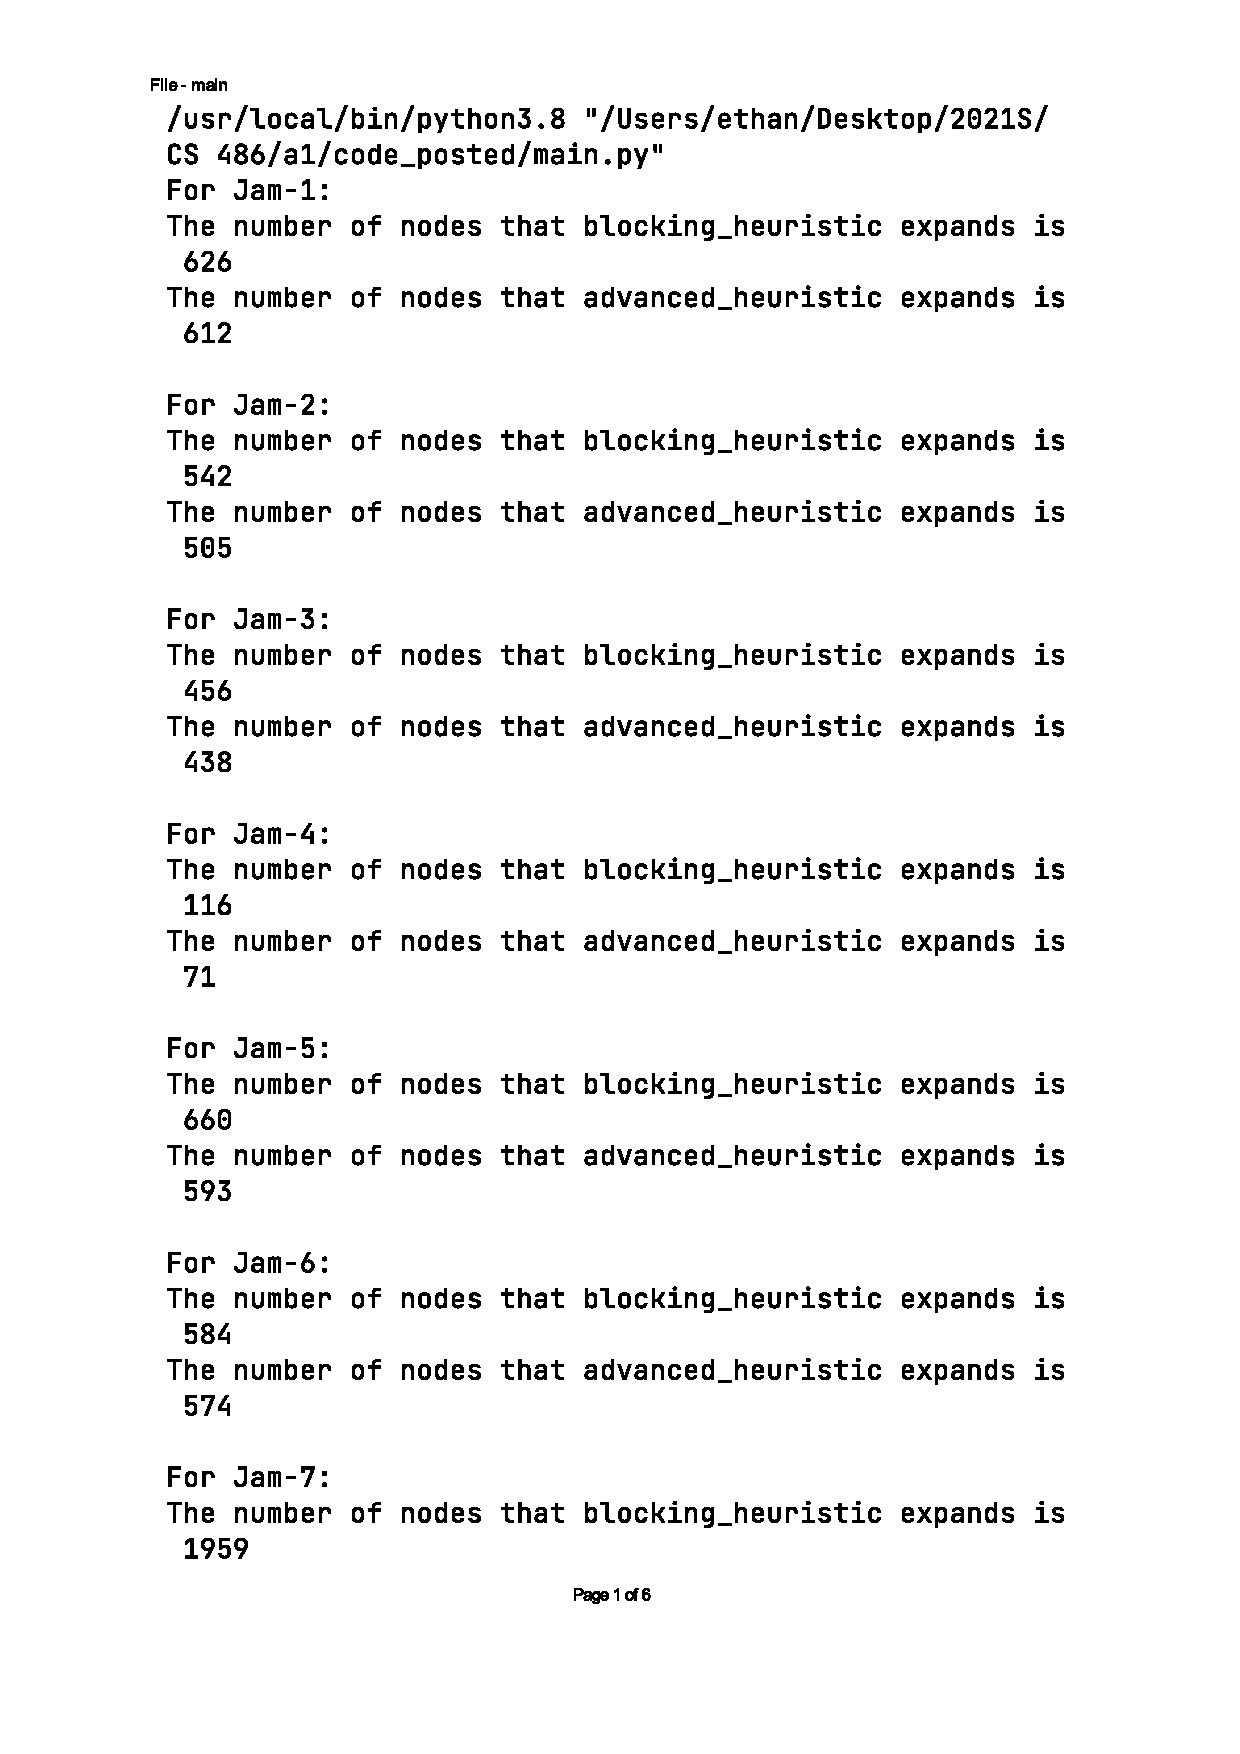
\includepdf[pages={1-},pagecommand=\appendixpage\appendix\label{appendix}, scale=0.8]{output.pdf}


\end{document}





























